
\section{pape - Wide-Angle Pade Parabolic Equation Code}
\label{sec: pape}

\subsection{Mathematical Background}
{\bf pape} uses the Parabolic Equation method (see chapter 6 of reference~\cite{comp_oc_ac}) to solve the single-frequency infrasound propagation in a range-dependent atmosphere over rigid ground in the limit of the effective sound speed approximation. Assuming that the pressure field has weak azimuthal dependence the coresponding Helmholtz equation is:
\[
\left[ \frac{1}{r} \frac{\partial}{\partial r} \left( r \frac{\partial}{\partial r} \right) 
+ 
\rho_0 \frac{\partial}{\partial z} \left( \frac{1}{\rho_0} \frac{\partial}{\partial z} \right) 
+ 
\Big(\frac{\omega}{c_{eff}}+i\alpha\Big)^2\right] p(r,z) 
= 
0
\]
where \( p(r,z) \) is the pressure deviation at range \(r\) and height \( z \), \(\omega \) is the angular frequency,  \(\rho_0 \) is the air density and \(c_{eff}\) is the effective (complex) sound speed i.e. the sum of the sound speed and the wind velocity component in the (horizontal) direction of wave propagation. The atmospheric absorption and damping of the acoustic energy is accounted for as the imaginary component of the wavenumber $\frac{\omega}{c}$. The pressure deviation satisfies the boundary condition 
\[
\frac {\partial p}{\partial z}\Big |_{z=0}= 0
\]
and the asymptotic condition 
\[
\lim_{r,(z-z_S)\downarrow0}\Big(p(r,z,\omega)-\frac{1}{\sqrt{r^2+(z-z_S)^2}}\Big)=0.
\]

It is assumed that the solution takes the form
\[
p(r,z) = \psi(r,z) H_0^{(1)}(k_0r)
\]
where $\psi(r,z)$ is a slowly varying with $r$ envelope and $k_0 =  {\omega}/ {c_0}$ is a reference wavenumber. Denoting the index of refraction $n(r,z) = c0/c(r,z))$ the equation to solve becomes:
\[
\frac {\partial^2 \psi}{\partial r^2} + 2ik_0 \frac {\partial \psi} {\partial r} 
+ 
\rho_0 \frac {\partial} {\partial z} \left( \frac {1} {\rho_0} \frac {\partial \psi} { \partial z}\right) 
+ 
k_0^2 (n^2 - 1) \psi = 0 . 
\]
This equation can be factored into two one-way equations, for forward propagating and back-propagating energy. Denoting the operators:
\[
Q = \rho_0 \frac {\partial} {\partial z} \left( \frac {1} {\rho_0} \frac {\partial } { \partial z}\right) + k_0^2 n^2  
\quad {\text{  and  } }  \quad
q = \frac {1} { k_0^2} (Q - k_0^2), 
\]
the one way forward-propagating wave equation is:
\begin{equation}
\frac {\partial \psi} {\partial z} = ik_0 \left( -1 + \sqrt {1 + q} \right) \psi .
\label{eq: pe 1-way eq}
\end{equation}
The square root operator in this last equation is implemented numerically with a Pade approximation of order $M$:
\[
\sqrt {1 + q} \approx 1 + \sum_{m=1}^M \frac {a_m q} { 1 + b_m q} , 
\]
where the coefficients are:
\[
a_m = \frac {2} { 2M+1} \sin^2 \frac {m \pi} { 2M + 1}, \quad   b_m =  \cos^2 \frac {m \pi} { 2M + 1}. 
\]
Equation~\ref{eq: pe 1-way eq} is then solved following the method described in section 6.6.2 of reference~\cite{comp_oc_ac}.


\subsection{Running pape}
\label{sec: running pape}

Making sure that the executable for {\bf pape} is in the system's path, it can be run by entering 
\begin{verbatim} 
    pape [--option1 val1] [--option2 val2] [...] [--flag1] [...] 
\end{verbatim}
on a command line. Generally, options are followed by values, either numbers, strings or filenames. Flags are not. Entering \verb"pape" without any options or flags sends the following help page to the screen: 

\begin{verbatim}
By default 'pape' computes the 1D transmission loss (TL)
at the ground or the specified receiver height and saves the data to:
   file tloss_1d.pe - considering attenuation in the atmosphere
Additionally, if the flag --write_2D_TLoss is given the 2D TL is saved 
to file tloss_2d.pe.

The options below can be specified in a colon-separated file "PAPE.options" 
or at the command line.  Command-line options override file options.
Be sure to precede the options with two minuses: --

 --help -h                Print this message and exit

 The atmosphere can be specified from one of 4 different sources:
    1. An .env file containing the atmospheric specifications at certain ranges:
       use option --g2senvfile <filename>
    2. Several ASCII files stored in a given directory:
       use option --use_1D_profiles_from_dir <mydirname>
    3. A single ASCII file. This will just force a range-independent run.
       use option --atmosfile1d <filename>
    4. A built-in NCPA canonical profile.
       use option (flag) --ncpatoy

The available options are:

REQUIRED (no default values):
 --atmosfileorder         The order of the (z,u,v,w,t,d,p) fields in the file
                          (Ex: 'ztuvpd')
 --skiplines              Lines at the beginning of the ASCII file to skip
 --azimuth                Degrees in range [0,360), clockwise from North
 --freq                   Frequency [Hz]
 --g2senvfile <filename>  Uses an .env binary file (for range-dependent code)
 --use_1D_profiles_from_dir
                          e.g. --use_1D_profiles_from_dir <myprofiles>
                          This option allows to use the ascii profiles stored in
                          the specified directory. The profiles must have names
                          'profiles0001', 'profiles0002', etc. and will be
                          used in alphabetical order at the provided ranges
                          e.g. in conjunction with either
                          option  '--use_profile_ranges_km' 
                          or option '--use_profiles_at_steps_km'
                          If there are more requested ranges than existing
                          profiles then the last profile is used repeatedly
                          as necessary.
    Example: >> ../bin/pape --atmosfileorder zuvwtdp --skiplines 1
                --azimuth 90 --freq 0.1 --use_1D_profiles_from_dir myprofiles_dir
                --use_profile_ranges_km 100_300_500_600_700

 --atmosfile1d  <filename>  Uses an ASCII 1D atmosphere file.
                          In this case the run will just be range-independent.

OPTIONAL [defaults]:
 --maxheight_km           Calculation grid height in km above MSL [150 km]
 --zground_km             Height of the ground level above MSL [0 km]
 --Nz_grid                Number of points on the z-grid from ground to maxheight [20000]
 --sourceheight_km        Source height in km Above Ground Level (AGL) [0]
 --receiverheight_km      Receiver height in km AGL [0]
 --maxrange_km            Maximum horiz. propagation distance from origin [1000 km]
 --rng_step               A usually fractional number specifying the range step
                          in wavelengths: e.g. --rng_step 0.1 means a step
                          of 0.1*wavelength [default is 0.1].
 --ground_impedance_model Name of the ground impedance models to be employed:
                          [rigid], others TBD
 --wind_units             Specify 'kmpersec' if the winds are given
                          in km/s [ mpersec ]
 --n_pade                 Number of Pade coefficients [4]

 --starter_type           Specifies one of 3 available PE starter
                          fields: gaussian, greene, modal.
                          The default is 'gaussian'.
                          'modal' requires a precomputed starter field
                          obtained by running Modess with option
                          --modal_starter_file.




 --use_profile_ranges_km
                          e.g. --use_profile_ranges_km  20_50_80.5_300     
                          The profiles at certain ranges specified by numbers
                          (in km) in a string such as 20_50_80.5_300 are
                          requested in the propagation. Note that underscores
                          are necessary to separate the numbers.
                          In this example the ranges at which the profiles
                          are considered are: 0, 20, 50, 80.5, 300 km i.e.
                          0 is always the first distance even if not specified.
                          Note also that these are requested ranges;
                          however the left-closest profile available
                          in the .env file will actually be used; 
                          for instance we request the profile at 300 km 
                          but in the .env file the left-closest profile
                          may be available at 290 km and it is the one used.
                          This convention may change in the future.
                          This option is used in conjunction with
                              --use_1D_profiles_from_dir

 --use_profiles_at_steps_km
                          e.g. --use_profiles_at_steps_km 100
                          The profiles are requested at equidistant intervals 
                          specified by this option [1000]
                          This option is used in conjunction with
                              --use_1D_profiles_from_dir

 --use_attn_file          Use it to specify a file name containing user-provided
                          attenuation coefficients to be loaded instead of 
                          the default Sutherland-Bass attenuation. 
                          The text file should contain two columns: 
                              height (km AGL) and 
                              attenuation coefficients in np/m.


FLAGS (no value required):
 --ncpatoy                Use built-in NCPA canonical profile
 --write_2D_TLoss         Outputs the 2D transmission loss to
                          default file: tloss_2d.pe
 --do_lossless            Computation is done with no atm. absorption


 The column order of the output files is as follows (P is complex pressure):
  tloss_1d.pe:           r, 4*PI*Re(P), 4*PI*Im(P)
  tloss_2d.pe:        r, z, 4*PI*Re(P), 4*PI*Im(P)


--------------------------------------------------------------------
Examples to run with various options (from the 'samples' directory):

    ../bin/pape  --ncpatoy --azimuth 90 --freq 0.1 --write_2D_TLoss

    ../bin/pape --g2senvfile g2sgcp2011012606L.jordan.env 
                --atmosfileorder zuvwtdp --skiplines 0 --azimuth 90 
                --freq 0.3 --sourceheight_km 0 --receiverheight_km 0 
                --maxheight_km 180 --starter_type gaussian --n_pade 6 
                --maxrange_km 500

    ../bin/pape --atmosfile1d NCPA_canonical_profile_zuvwtdp.dat 
                --atmosfileorder zuvwtdp --skiplines 0 --azimuth 90 --freq 0.1 
                --sourceheight_km 0 --receiverheight_km 0 --maxheight_km 180 
                --starter_type gaussian --n_pade 4 --maxrange_km 500

    ../bin/pape --use_1D_profiles_from_dir ../samples/profiles 
                --atmosfileorder zuvwtdp --skiplines 1 --azimuth 90 --freq 0.1 
                --sourceheight_km 0 --receiverheight_km 0 --maxheight_km 180
                --starter_type gaussian --n_pade 6 --maxrange_km 1000  
                --use_profiles_at_steps_km 20

    ../bin/pape --use_1D_profiles_from_dir ../samples/profiles 
                --atmosfileorder zuvwtdp --skiplines 1 --azimuth 90 --freq 0.1 
                --sourceheight_km 0 --receiverheight_km 0 --maxheight_km 180 
                --starter_type gaussian --n_pade 6 --maxrange_km 1000  
                --use_profile_ranges_km 0_20_60_400
\end{verbatim}

The functionality of {\bf pape} is much like that of {\bf ModessRD1WCM}, see section~\ref{sec:running modbb}. In particular, the input of atmospheric profiles is much the same, with the exception that {\bf pape} has a flag for the use of the NCPA toy model. Further, if a G2S {\tt .env} file is used as input the set of atmospheric profiles are read in order from the {\tt .env} file itself; \verb+--use_profile_ranges_km+ and \verb+--use_profiles_at_steps_km+ have no effect. The two programs share the same options and flags with some exceptions. Like all PE models, {\bf pape} requires the use of a starter to simulate a near field source function. {\bf pape} supports the use of a Gaussian starter, a Greens function starter and a modal starter. The Modal starter requires that there be a modal starter file that can be created with {\bf Modess}. The option \verb+--rng_step+ sets the step size in the PE's marching scheme in fractions of a wavelength. One may use \verb+--n_pade+ to set the order of the Pade approximation to use. In addition, to run {\bf pape} without attenuation requires the use of the flag \verb+--do_lossless+. 

\subsection{Running pape: examples}
\label{sec: pade examples}

\begin{figure}[h]
\begin{center}
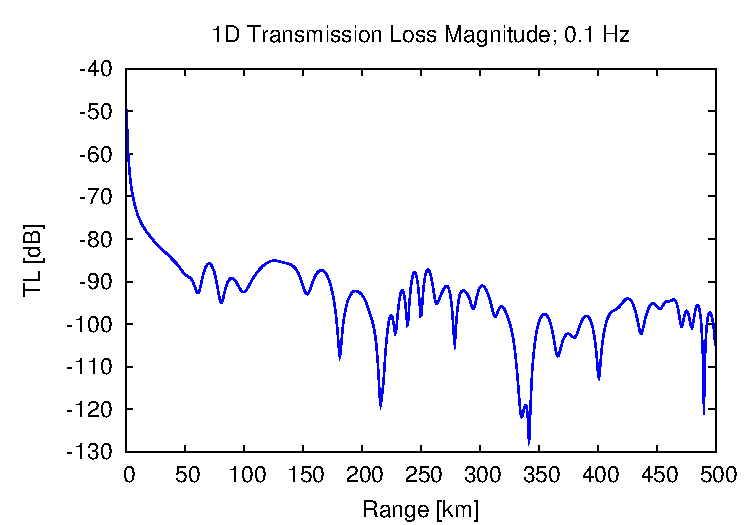
\includegraphics[scale=0.60]{figs/pade_ex1_1d}
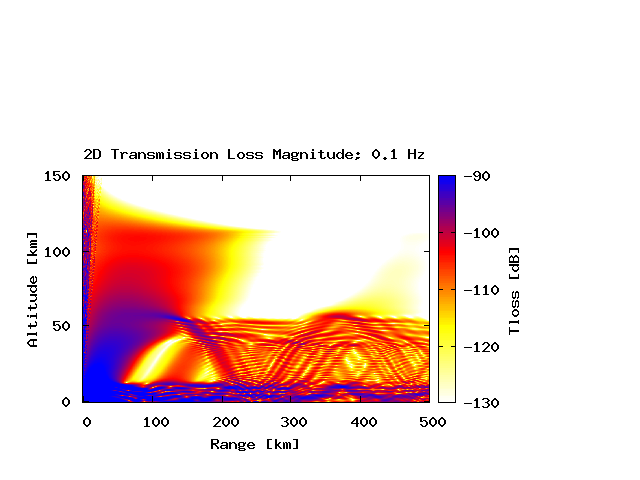
\includegraphics[scale=0.45,trim = 20 20 110 140,clip]{figs/pade_ex1_2d.png}
\end{center}
\caption{1D transmission loss magnitude at 0.3 Hz obtained with {\bf pade} for eastward ground-to-ground propagation in the range dependant profiles provided by a G2S {\tt .env} binary file. Shown are the 1D lossless transmission loss magnitude and lossy transmission loss magnitude and the 2D lossy transmission loss magnitude.}
\label{fig: pade ex1}
\end{figure}

The following example illustrates the functionality and inputs of ModessRD1WCM using a user-provided G2S {\tt .env} file. 
\begin{verbatim}
    ../bin/pape --g2senvfile g2sgcp2011012606L.jordan.env 
                --atmosfileorder zuvwtdp --skiplines 0 --azimuth 90 
                --freq 0.3 --sourceheight_km 0 --receiverheight_km 0 
                --maxheight_km 180 --starter_type gaussian --n_pade 6 
                --maxrange_km 500
\end{verbatim}
The resulting data files are plotted in Figure \ref{fig: pade ex1}. 

\begin{figure}[h]
\begin{center}
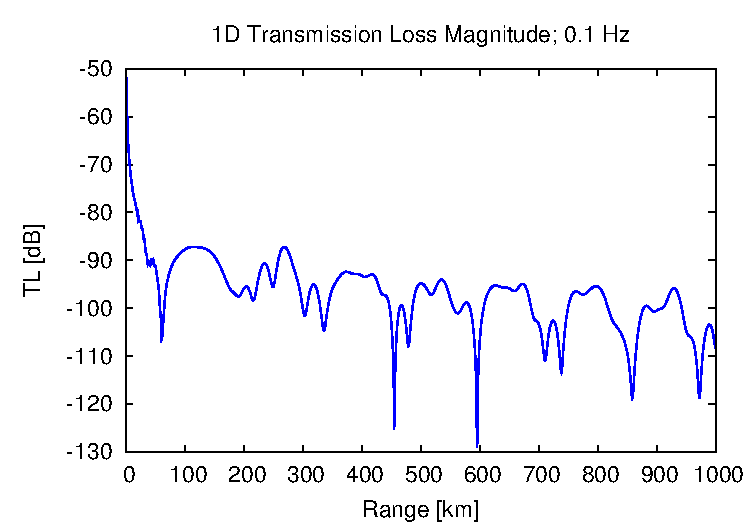
\includegraphics[scale=0.60]{figs/pade_ex2_1d}
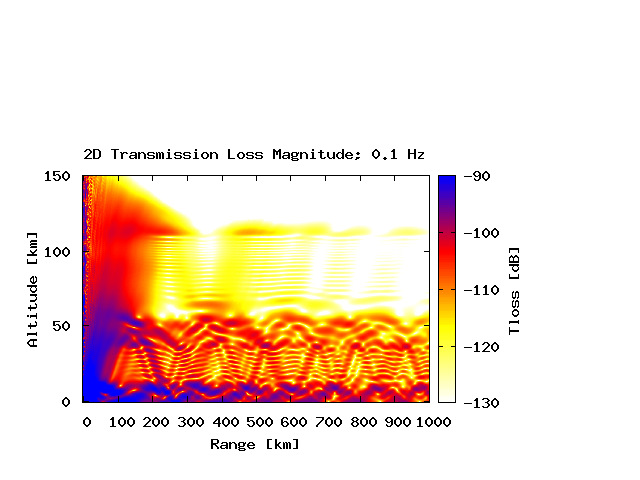
\includegraphics[scale=0.45,trim = 20 20 110 140,clip]{figs/pade_ex2_2d.png}
\end{center}
\caption{1D transmission loss magnitude at 0.1 Hz obtained with {\bf pade} for eastward ground-to-ground propagation in the range dependant profiles provided in the directory {\tt profiles}. Shown are the 1D lossless transmission loss magnitude and lossy transmission loss magnitude and the 2D lossy transmission loss magnitude.}
\label{fig: pade ex2}
\end{figure}

The following example illustrates the functionality and inputs of ModessRD1WCM using user-provided range dependant atmospheric profiles provided by a directory of one-dimensional ascii files. 
\begin{verbatim}
    ../bin/pape --use_1D_profiles_from_dir profiles 
                --atmosfileorder zuvwtdp --skiplines 1 --azimuth 90 --freq 0.1 
                --sourceheight_km 0 --receiverheight_km 0 --maxheight_km 180 
                --starter_type gaussian --n_pade 6 --maxrange_km 1000  
                --use_profile_ranges_km 0_20_60_400
\end{verbatim}
The resulting data files are plotted in Figure \ref{fig: pade ex2}. 


\subsection{tdpape - Time Domain Pade Parabolic Equation}

{\bf tdpape} provides Fourier synthesis of broad band signals using frequency-domain solutions obtained with \verb"pape". It has functionality similar to {\bf ModBB} (section~\ref{sec:running modbb}) except that range dependant atmospheric profiles are supported. See Chapter 8 of reference~\cite{comp_oc_ac} for more details on Fourier synthesis of broad band signals.  

\subsection{Running tdpape}

To run {\bf tdpape} make sure its executable is in the system's path and enter 
\begin{verbatim} 
    tdpape [--option1 val1] [--option2 val2] [...] [--flag1] [...] 
\end{verbatim}
on a command line. Generally, options are followed by values, either numbers, strings or filenames. Flags are generally not. Entering \verb"tdpape" without any options or flags sends the following help page to the screen: 

\begin{verbatim}
The options below can be specified at the command line or in a colon-separated
file "tdpape.options". Command-line options override file options.
Be sure to precede all options with two minuses (--).

 --help -h                Print this message and exit


To propagate a pulse (waveform), 2 steps must be completed:
 1. Pre-computed single-frequency output files from pape must be available
    and stored in the same directory. If N frequencies were computed
    the template for the file names is
    <#n>papeTL<freq>; e.g. 004_papeTL_0.87776
    Please refer to script xrun_papeBB.sh for an example on how to
    compute single-frequency files in batch mode. 

 2. Perform pulse propagation for 2 scenarios:
    a. source-to-one-receiver at one range (see option --pulse_prop_src2rcv)
    b. source-to-several-receivers at equally spaced ranges (i.e. on a grid)
       (see option --pulse_prop_src2rcv_grid)

 Output:  
    The text output file has the column order:
    for option --pulse_prop_src2rcv: | Time (seconds) | Waveform | 
    for option --pulse_prop_src2rcv_grid:
    | Range [km] | Time [seconds] | Waveform |
    Here 'Range' changes to reflect all receiver ranges on the defined grid.

 Four types of sources are available:
       delta function              -> see option --get_impulse_resp
       built-in pulse              -> see option --use_builtin_pulse
       user-provided spectrum file -> see option --src_spectrum_file
       user-provided waveform file -> see option --src_waveform_file


Options:
 --pulse_prop_src2rcv <directory name of pre-computed pape files> 
                    Propagate pulse from source to 1 receiver
                    at a distance specified by option --range_R_km; 
 --range_R_km       Propagate pulse to this range [km]
 --waveform_out_file <waveform filename>   Name of the waveform output file.

 --pulse_prop_src2rcv_grid <directory name of pre-computed pape files>
                    Propagate pulse from source to array of 
                    horizontally equally-spaced receivers

 REQUIRED additional options:
 --R_start_km       Propagation from this range to R_end_km in DR_km steps.
 --R_end_km         Pulse is propagated from R_start_km to this range.
 --DR_km            Range step to propagate from R_start_km to R_end_km.

 OPTIONAL [defaults]:
 --max_celerity     Maximum celerity [300 m/s].
 --f_center         The center frequency of the pulse; must be <= [f_max/5].

SOURCE TYPE options: Use one of the following 4 options to specify the source:
 --get_impulse_resp       Flag to use a (band-limited) delta function as source and
                          to output the impulse response (this is the default).
 --use_builtin_pulse      Flag to request the use of the built-in source pulse.
 --src_spectrum_file      Specify the file name of the source spectrum
                          at positive frequencies. The file must have 3 columns
                             | Freq | Real(Spectrum) | Imag(Spectrum) |
 --src_waveform_file      Specify the file name of the user-provided 
                          source waveform. The file must have 2 columns
                             |Time | Amplitude |
   If none of then source type options are specified the delta function source
   is the default i.e. the output is the impulse response.

 QUICK-START EXAMPLES (run from the 'samples' directory):
 (Assume that the pre-computed single frequency files reside in myTDPape_dir.) 

 Example 1: Pulse propagation to a point on the ground at range_R_km
            and output the impulse response:

    ../bin/tdpape --pulse_prop_src2rcv myTDPape_dir --range_R_km 240 
                  --waveform_out_file mywavf.dat --max_celerity 320 --get_impulse_resp

 Example 2: Pulse propagation to a point on the ground at range_R_km
            and employ the built-in source pulse:

    ../bin/tdpape --pulse_prop_src2rcv myTDPape_dir --range_R_km 240 
              --waveform_out_file mywavef.dat --max_celerity 320 --use_builtin_pulse

 Example 3: Pulse propagation to several points on the ground 20 km apart
            and employ the user-provided source waveform:

    ../bin/tdpape --pulse_prop_src2rcv_grid  myTDPape_dir  
              --R_start_km 200 --R_end_km 240 --DR_km 20 
              --waveform_out_file mywavef.dat --max_celerity 320 
              --src_waveform_file source_waveform_input_example.dat

 Example 4: Pulse propagation to a point on the ground at range_R_km
            and employ the user-provided source spectrum:

    ../bin/tdpape --pulse_prop_src2rcv myTDPape_dir --range_R_km 240 
                --waveform_out_file mywavf.dat --max_celerity 320 
                --src_spectrum_file source_spectrum_example.dat
\end{verbatim}

\subsection{Running tdpape: example}

Here is a simple example run to illustrate the main input for \verb+tdpape+.
\begin{verbatim} 
    ../bin/tdpape --pulse_prop_src2rcv myTDPape_dir --range_R_km 240 
                  --waveform_out_file mywavf.dat --max_celerity 320 --get_impulse_resp
\end{verbatim}

In this example the impulse response for ground to ground propagation to a receiver at range = 240 km is calculated. 

The directory \verb"myTDPapedir" should contain single-frequency output files from \verb"pape" covering the spectrum band desired. Assuming that band of interest contains N frequencies the template for the file names is  \verb"<#n>_papeTL_<freq>"  e.g. \verb"004_papeTL_0.87776".  The script \verb"xrun_papeBB.sh" is a shell script providing an example on running \verb"pape" in batch mode and storing single frequency output in the a desired directory (e.g.\verb"myTDpape_dir").

